\section{Theorie}
\label{sec:Theorie}

\subsection {Gedämpfte Schwingungen}
Besteht ein Schaltkreis aus einer Induktivität $L$, realisiert durch eine Spule, und einem Kondensator mit der Kapaziät $C$, führt das System
ungedämpfte Schwingungen durch. Die Energie pendelt zwischen den Speichern hin und her und führt deshalb periodische Schwingungen durch.
Wird dem Schaltkreis ein ohmscher Widerstand $R$ hinzugefügt, nimmt die Energie mit der Zeit ab, die Amplituden von Strom und Spannung fallen,
und das System führt Gedämpfte Schwingungen aus. Ein Aufbau eines solches Schwingkreises ist in Abbildung (1) dargestellt. Dieses System führt
\begin{figure}[H]
  \centering
  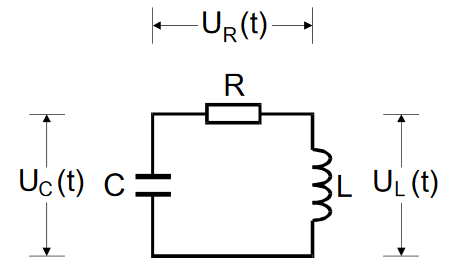
\includegraphics[height=5cm]{RLC.png}
  \caption{Aufbau eins RLC-Schwingkreises. \cite[S.1]{kent}}
\end{figure}
\noindent Mit Hilfe des 2. Kirchhoffschen Gesetzes kann man die Differentialgleichung für den Schaltkreis aufstellen.
\begin{equation}
U_R (t) + U_C (t) + U_L (t) = 0 .
\end{equation}
Setzt man die Gleichungen
\begin{align}
U_R (t) = R I(t)  \\
U_C (t) = \frac{Q(t)}{C}  \\
U_L (t) = L \frac{dI}{dt} \\
I = \frac{dQ}{dt}
\end{align}
mit $Q(t)$ als Ladung in die DGL ein, und leitet einmal ab, ergibt sich 
\begin{equation}
\frac{d^2I}{dt^2} + \frac{R}{L}\frac{dI}{dt} + \frac{1}{LC}I = 0 .
\end{equation}
Setzt man den Ansatz
\begin{equation*}
I(t) = U e^{j\omega t}
\end{equation*}
in die DGL ein, ergibt sich die charakteristiche Gleichung
\begin{equation}
\omega^{2} - j\frac{R}{L}\omega - \frac{1}{LC} = 0 
\end{equation}
\noindent mit 
\begin{equation}
\omega_{1,2} = j \frac{R}{2L} \pm \sqrt{\frac{1}{LC} - \frac{R^{2}}{4L^{2}}} .
\end{equation}
\noindent Die Gleichung lässt sich schreiben als 
\begin{equation}
I(t) = e^{-2\pi \mu t}(U_1 e^{j2\pi \nu t} + U_2 e^{-j2\pi \nu t})
\end{equation}
\noindent mit den Abkürzungen 
\begin{align}
2\pi \mu = \frac{R}{2L} \\
&2\pi \nu = \sqrt{\frac{1}{LC} - \frac{R^{2}}{4L^{2}}} .
\end{align}
\noindent Je nachdem ob $\frac{1}{LC}$ größer oder kleiner $\frac{R^2}{4L^2]}$ ist, also $\nu$ reell oder imaginär ist,
sieht $I(t)$ anders aus. Somit muss eine Fallunterscheidung getroffen werden.
Im Ersten Fall sei $\nu$ reell. Die DGL ergibt sich dann zu
\begin{equation}
I(t) = Ae^{-2\pi \mu t}cos(2\pi \nu t + \eta) .
\end{equation}
Man erkennt, dass diese Gleichung eine harmonische Schwingung beschreibt, mit $\nu$ als Frequenz, und exponentiell abklingender Amplitude.
Sie stellt die gedämpfte Schwingung dar. Die Abklingdauer dieser Schwingung, bestimmt sich durch
\begin{equation}
T_{ex} = \frac{1}{2\pi \mu} = \frac{2L}{R} ,
\end{equation}
und nach dieser hat die Amplitude ihren ursprünglichen Wert angenommen.
Darstellen lässt sich eine gedämpfte Schwingung durch die Abbildung (2).
\begin{figure}[H]
  \centering
  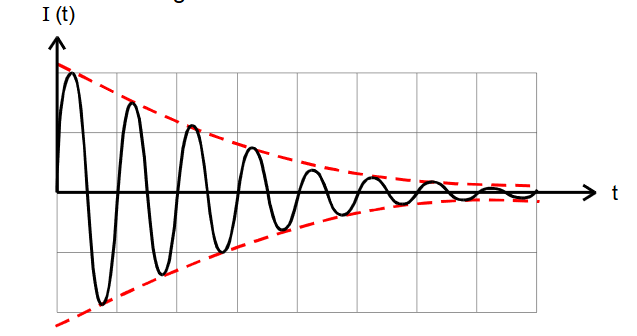
\includegraphics[height=5cm]{grenzfall.png}
  \caption{Darstellung einer gedämpften Schwingung. \cite[S.4]{kent}}
\end{figure}
\noindent Betrachtet man nun den zweiten fall, also dass $\nu$ imaginär ist, verhält sich die Schwingung nicht mehr oszillatorisch, und die aperiodische Dämpfung tritt ein.
Die aperiodische Dämpfung ist in Abbildung (3) dargestellt. $I(t)$ nähert sich in diesem Fall am schnellsten null an.
Es gilt dann außerdem
\begin{equation}
I(t) \propto e^{-(2\pi \mu - i2\pi \nu)t} .
\end{equation}
Gilt
\begin{equation}
\frac{1}{LC} = \frac{R_{ap}^2}{4L^2} ,
\end{equation}
ergibt sich die DGL zu
\begin{equation}
I(t) = A e^{-\frac{t}{\sqrt{LC}}} .
\end{equation}
\begin{figure}[H]
  \centering
  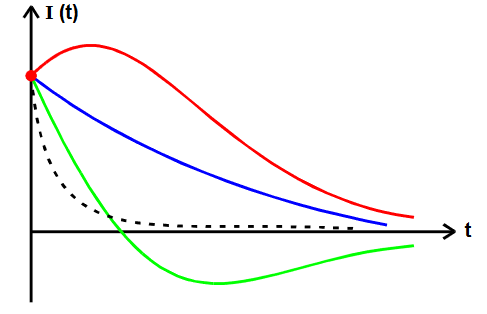
\includegraphics[height=5cm]{aperiodisch.png}
  \caption{Darstellung des aperiodischen Grenzfalls. \cite[S.5]{kent}}
\end{figure}



\subsection{Erzwungene Schwingungen}
Wirkt an einen Schwingkreis eine äußere periodische Kraft, führt das System erzwungene Schwingungen aus.
Wird zum Beispiel eine Sinusspannung als Spannungsquelle eingeschaltet, wie in Abbildung (4) zu sehen ist,
nimmt die Differentialgleichung folgende Gestalt an:
\begin{equation}
LC\frac{d^2 U_C}{dt^2} + RC\frac{d U_C}{dt} + U_C = U_0 e^{j\omega t} .
\end{equation}
Die Lösung dieser Gleichung lautet
\begin{equation}
U = \frac{U_0(1-LC\omega^2 - j\omega RC)}{(1-LC\omega^2)^2 + \omega^2 R^2 C^2} .
\end{equation}
Die zugehörige Phase wird durch 
\begin{equation}
\phi(\omega) = arctan(\frac{-\omega RC}{1-LC\omega^2})
\end{equation}
beschrieben.
Die Resonanzkurve, also die Abhängigkeit der Kondensatorspannung $U_C$ von der Frequenz der Erregerspannung, wird durch
\begin{equation}
U_C(\omega) = \frac{U_0}{\sqrt{(1-LC\omega^2)^2 + \omega^2 R^2 C^2}}
\end{equation}
beschrieben. $U_C$ kann bei einer endlichen Frequenz ein Maximum erreichen, welches als Resonanz mit Resonanzfrequenz $\omega_{res}$ bezeichnet wird.
Diese lautet
\begin{equation}
\omega_{res} = \sqrt{\frac{1}{LC} - \frac{R^2}{2L^2}} .
\end{equation}
Im Falle der schwachen Dämpfung
\begin{align*}
\frac{R^2}{2L^2} \ll \frac{1}{LC}
\end{align*}
Kann $U_C$ die Spannung $U_0$ um den Gütefaktor $\frac{1}{\omega_0 RC}$ übertreffen 
\begin{equation}
U_{C,max} = \frac{1}{\omega_0 RC}U_0
\end{equation}
und gegen unendlich gehen, liegt die Resonanzkatastrophe vor.
Die Schärfe der Resonanz kann man durch die Breite der Resonanzkurve beschrieben, für welche gilt:
\begin{align*}
\omega _+ - \omega _- \approx \frac{R}{L} .
\end{align*}
\begin{figure}[H]
  \centering
  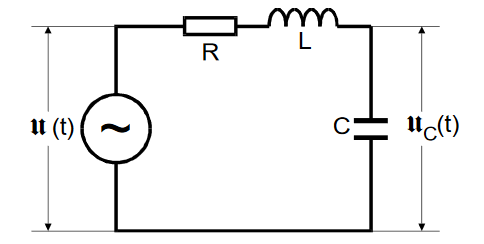
\includegraphics[height=5cm]{erzwungen.png}
  \caption{Schaltung mit einer Sinusspannung als Spannungsquelle. \cite[S.6]{kent}}
\end{figure}
